\section{Parallelization}
\label{sec:parllel}

\begin{frame}
    \frametitle{Parallelization}

    \begin{columns}
        \begin{column}{0.5\textwidth}
            \centerline{
                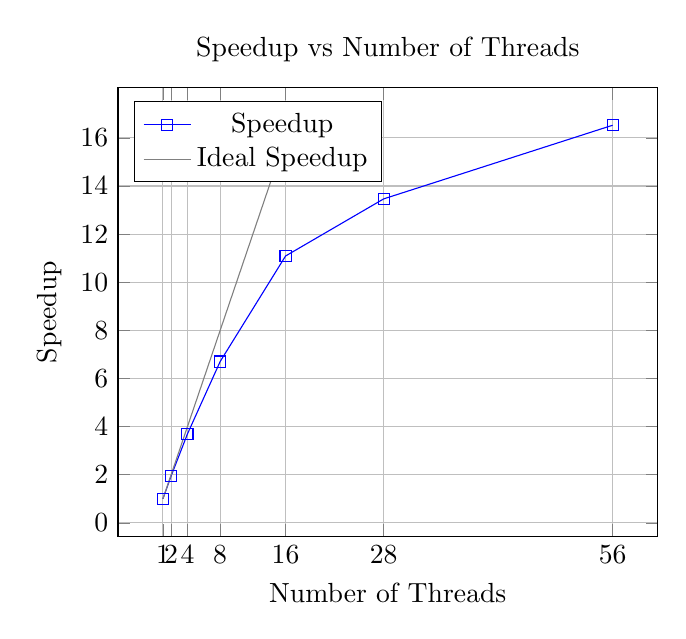
\begin{tikzpicture}
                \begin{axis}[
                    title={Speedup vs Number of Threads},
                    xlabel={Number of Threads},
                    ylabel={Speedup},
                    grid=both,
                    xtick={1, 2, 4, 8, 16, 28, 56},
                    ytick={0, 2, 4, 6, 8, 10, 12, 14, 16},
                    legend pos=north west
                ]
                \addplot[
                    color=blue,
                    mark=square,
                    ]
                    coordinates {
                    (1, 1)
                    (2, 3272 / 1680)
                    (4, 3272 / 885)
                    (8, 3272 / 488)
                    (16, 3272 / 295)
                    (28, 3272 / 243)
                    (56, 3272 / 198)
                    };

                    \addplot[
                    color=gray,
                    ]
                    coordinates {
                    (1, 1)
                    (16, 16)
                    };
                \addlegendentry{Speedup}
                \addlegendentry{Ideal Speedup}
                \end{axis}
                \end{tikzpicture}
            }
        \end{column}
            \begin{column}{0.5\textwidth}
                \begin{figure}
                    \centering
                    \includegraphics[width=\columnwidth]{../../res/optimized.png}
                    \caption{Visualization of runtime distributions.}
                    \label{fig:runtime}
                \end{figure}
            \end{column}
    \end{columns}


\end{frame}